\section{Opis Modelu SI}\label{sec:opis-modelu-si}

Model sztucznej inteligencji został zaprojektowany w celu klasyfikacji zdjęć ośmiościennych kości do jednej z ośmiu klas, odpowiadających cyfrom od 1 do 8.
Do implementacji modelu wykorzystano moduły scikit-learn oraz wchodzący w jego skład Keras, obecnie jako część modułu Tensorflow, który umożliwia łatwe tworzenie i trenowanie sieci neuronowych.
\textit{Biblioteka Keras jest wygodnym opakowaniem (wrapperem) dla modeli DL używanych do oszacowań klasyfikacji lub regresji]} [Donald J. Norris, 2020 s. 355 wydanie APN PROMISE SA]

\subsection{Przygotowanie danych}\label{subsec:przygotowanie-danych}

Dane wejściowe zostały podzielone na zestawy treningowy i walidacyjny w proporcji 70:30.
W celu zwiększenia różnorodności danych treningowych zastosowano techniki augmentacji obrazów, takie jak:

\begin{itemize}
    \item obrót o losowy kąt w zakresie do 90°,
    \item przesunięcia poziome i pionowe,
    \item transformacje perspektywiczne (shear) ,
    \item losowe powiększenia (zoom) .
\end{itemize}

Przykład konfiguracji generatora danych:

\begin{verbatim}
datagen = ImageDataGenerator(
    rescale=1.0 / 255.0,
    validation_split=0.3,
    rotation_range=90,
    width_shift_range=0.2,
    height_shift_range=0.2,
    shear_range=0.1,
    zoom_range=0.1
)
\end{verbatim}

\subsection{Architektura modelu}\label{subsec:architektura-modelu}

Model jest wielowarstwową siecią konwolucyjną (CNN) składającą się z następujących elementów:

\begin{itemize}
    \item Warstwy wejściowej
    \begin {verbatim}
    layers.Input(shape=(64, 64, 1))
    \end {verbatim}
    \item Trzech warstw konwolucyjnych z funkcją aktywacji ReLU:
    \begin{verbatim}
    layers.Conv2D(32, (3, 3), activation='relu')
    layers.MaxPooling2D((2, 2))
    \end{verbatim}
    \item Warstwy spłaszczającej (Flatten),
    \item Dwóch w pełni połączonych warstw (Dense), z których ostatnia używa funkcji aktywacji softmax do klasyfikacji na 8 klas:
    \begin{verbatim}
    layers.Dense(128, activation='relu')
    layers.Dense(8, activation='softmax')
    \end{verbatim}
\end{itemize}

\subsection{Trenowanie modelu}\label{subsec:trenowanie-modelu}

Model został skompilowany z wykorzystaniem optymalizatora Adam, funkcji strat sparse categorical crossentropy oraz metryki dokładności.
Proces trenowania obejmował 20 epok:

\begin{verbatim}
model.compile(
    optimizer='adam',
    loss='sparse_categorical_crossentropy',
    metrics=['accuracy']
)
history = model.fit(
    train_data,
    validation_data=val_data,
    epochs=20,
    steps_per_epoch=train_data.samples,
    validation_steps=val_data.samples
)
\end{verbatim}

\subsection{Wyniki}\label{subsec:wyniki}

Podczas trenowania osiągnięto następujące końcowe wyniki:

\begin{itemize}
    \item Dokładność na zbiorze treningowym: 0,9375 \texttt{final\_train\_acc},
    \item Dokładność na zbiorze walidacyjnym: 1,0  \texttt{final\_val\_acc},
    \item Strata na zbiorze treningowym: 0,0786  \texttt{final\_train\_loss},
    \item Strata na zbiorze walidacyjnym: 0,0274  \texttt{final\_val\_loss}.
\end{itemize}

Wyniki zostały również zwizualizowane na wykresach przedstawiających zmianę dokładności i straty w trakcie trenowania.

\begin{figure}[H]
    \centering
    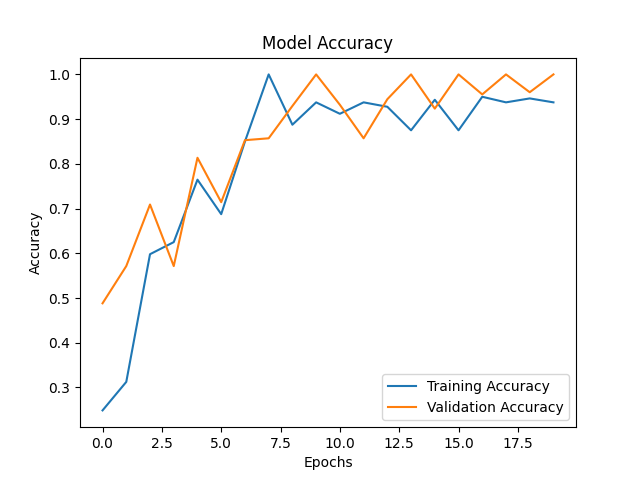
\includegraphics[width=0.8\textwidth]{chapters/04-czytanie/figures/ModelAcc1}
    \caption{Wykres dokładności modelu.}
    \label{fig:ModelAcc}
\end{figure}

\begin{figure}[H]
    \centering
    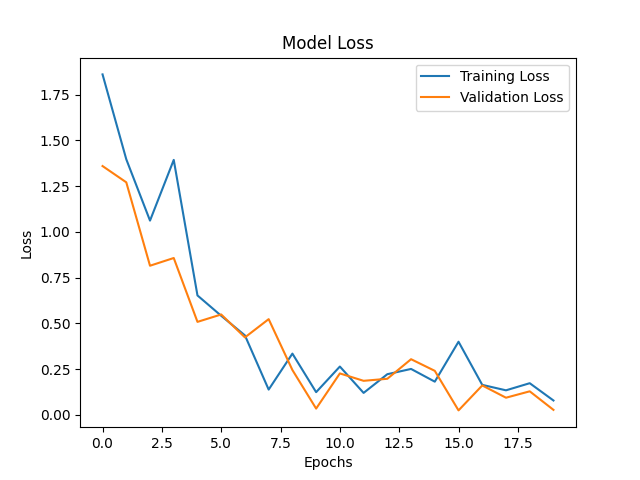
\includegraphics[width=0.8\textwidth]{chapters/04-czytanie/figures/ModelLoss1}
    \caption{Wykres straty modelu.}
    \label{fig:ModelLoss}
\end{figure}

Model został zapisany w formacie \texttt{keras} i jest gotowy do użycia w systemie rozpoznawania liczb na ośmiościennej kości, opisanym w kolejnej sekcji.

